%File: anonymous-submission-latex-2026.tex
\documentclass[letterpaper]{article} % DO NOT CHANGE THIS
\usepackage[submission]{aaai2026}  % DO NOT CHANGE THIS
\usepackage{times}  % DO NOT CHANGE THIS
\usepackage{helvet}  % DO NOT CHANGE THIS
\usepackage{courier}  % DO NOT CHANGE THIS
\usepackage[hyphens]{url}  % DO NOT CHANGE THIS
\usepackage{graphicx} % DO NOT CHANGE THIS
\urlstyle{rm} % DO NOT CHANGE THIS
\def\UrlFont{\rm}  % DO NOT CHANGE THIS
\usepackage{natbib}  % DO NOT CHANGE THIS AND DO NOT ADD ANY OPTIONS TO IT
\usepackage{caption} % DO NOT CHANGE THIS AND DO NOT ADD ANY OPTIONS TO IT
\frenchspacing  % DO NOT CHANGE THIS
\setlength{\pdfpagewidth}{8.5in} % DO NOT CHANGE THIS
\setlength{\pdfpageheight}{11in} % DO NOT CHANGE THIS
%
% These are recommended to typeset algorithms but not required. See the subsubsection on algorithms. Remove them if you don't have algorithms in your paper.
\usepackage{algorithm}
\usepackage{algorithmic}
\usepackage{booktabs}
\usepackage{multirow}
\usepackage{graphicx}
\usepackage{booktabs}
\usepackage{amsmath} % 自己加的包  用于在数学模式中插入普通文本
\usepackage{amssymb} % 自己加的包  用于打出“黑板粗体”
\usepackage{subcaption}

%
% These are are recommended to typeset listings but not required. See the subsubsection on listing. Remove this block if you don't have listings in your paper.
\usepackage{newfloat}
\usepackage{listings}
\DeclareCaptionStyle{ruled}{labelfont=normalfont,labelsep=colon,strut=off} % DO NOT CHANGE THIS
\lstset{%
	basicstyle={\footnotesize\ttfamily},% footnotesize acceptable for monospace
	numbers=left,numberstyle=\footnotesize,xleftmargin=2em,% show line numbers, remove this entire line if you don't want the numbers.
	aboveskip=0pt,belowskip=0pt,%
	showstringspaces=false,tabsize=2,breaklines=true}
\floatstyle{ruled}
\newfloat{listing}{tb}{lst}{}
\floatname{listing}{Listing}
%
% Keep the \pdfinfo as shown here. There's no need
% for you to add the /Title and /Author tags.
\pdfinfo{
/TemplateVersion (2026.1)
}

% DISALLOWED PACKAGES
% \usepackage{authblk} -- This package is specifically forbidden
% \usepackage{balance} -- This package is specifically forbidden
% \usepackage{color (if used in text)
% \usepackage{CJK} -- This package is specifically forbidden
% \usepackage{float} -- This package is specifically forbidden
% \usepackage{flushend} -- This package is specifically forbidden
% \usepackage{fontenc} -- This package is specifically forbidden
% \usepackage{fullpage} -- This package is specifically forbidden
% \usepackage{geometry} -- This package is specifically forbidden
% \usepackage{grffile} -- This package is specifically forbidden
% \usepackage{hyperref} -- This package is specifically forbidden
% \usepackage{navigator} -- This package is specifically forbidden
% (or any other package that embeds links such as navigator or hyperref)
% \indentfirst} -- This package is specifically forbidden
% \layout} -- This package is specifically forbidden
% \multicol} -- This package is specifically forbidden
% \nameref} -- This package is specifically forbidden
% \usepackage{savetrees} -- This package is specifically forbidden
% \usepackage{setspace} -- This package is specifically forbidden
% \usepackage{stfloats} -- This package is specifically forbidden
% \usepackage{tabu} -- This package is specifically forbidden
% \usepackage{titlesec} -- This package is specifically forbidden
% \usepackage{tocbibind} -- This package is specifically forbidden
% \usepackage{ulem} -- This package is specifically forbidden
% \usepackage{wrapfig} -- This package is specifically forbidden
% DISALLOWED COMMANDS
% \nocopyright -- Your paper will not be published if you use this command
% \addtolength -- This command may not be used
% \balance -- This command may not be used
% \baselinestretch -- Your paper will not be published if you use this command
% \clearpage -- No page breaks of any kind may be used for the final version of your paper
% \columnsep -- This command may not be used
% \newpage -- No page breaks of any kind may be used for the final version of your paper
% \pagebreak -- No page breaks of any kind may be used for the final version of your paperr
% \pagestyle -- This command may not be used
% \tiny -- This is not an acceptable font size.
% \vspace{- -- No negative value may be used in proximity of a caption, figure, table, section, subsection, subsubsection, or reference
% \vskip{- -- No negative value may be used to alter spacing above or below a caption, figure, table, section, subsection, subsubsection, or reference

\setcounter{secnumdepth}{0} %May be changed to 1 or 2 if section numbers are desired.

% The file aaai2026.sty is the style file for AAAI Press
% proceedings, working notes, and technical reports.
%

% Title

% Your title must be in mixed case, not sentence case.
% That means all verbs (including short verbs like be, is, using,and go),
% nouns, adverbs, adjectives should be capitalized, including both words in hyphenated terms, while
% articles, conjunctions, and prepositions are lower case unless they
\title{Appendix for MultiMedEdit: A Scenario-Aware Benchmark for Evaluating
Knowledge Editing in Medical VQA}
\author{
    %Authors
    % All authors must be in the same font size and format.
    Written by AAAI Press Staff\textsuperscript{\rm 1}\thanks{With help from the AAAI Publications Committee.}\\
    AAAI Style Contributions by Pater Patel Schneider,
    Sunil Issar,\\
    J. Scott Penberthy,
    George Ferguson,
    Hans Guesgen,
    Francisco Cruz\equalcontrib,
    Marc Pujol-Gonzalez\equalcontrib
}
\affiliations{
    %Afiliations
    \textsuperscript{\rm 1}Association for the Advancement of Artificial Intelligence\\
    % If you have multiple authors and multiple affiliations
    % use superscripts in text and roman font to identify them.
    % For example,

    % Sunil Issar\textsuperscript{\rm 2},
    % J. Scott Penberthy\textsuperscript{\rm 3},
    % George Ferguson\textsuperscript{\rm 4},
    % Hans Guesgen\textsuperscript{\rm 5}
    % Note that the comma should be placed after the superscript

    1101 Pennsylvania Ave, NW Suite 300\\
    Washington, DC 20004 USA\\
    % email address must be in roman text type, not monospace or sans serif
    proceedings-questions@aaai.org
%
% See more examples next
}

%Example, Single Author, ->> remove \iffalse,\fi and place them surrounding AAAI title to use it
\iffalse
\title{My Publication Title --- Single Author}
\author {
    Author Name
}
\affiliations{
    Affiliation\\
    Affiliation Line 2\\
    name@example.com
}
\fi

\iffalse
%Example, Multiple Authors, ->> remove \iffalse,\fi and place them surrounding AAAI title to use it
\title{My Publication Title --- Multiple Authors}
\author {
    % Authors
    First Author Name\textsuperscript{\rm 1},
    Second Author Name\textsuperscript{\rm 2},
    Third Author Name\textsuperscript{\rm 1}
}
\affiliations {
    % Affiliations
    \textsuperscript{\rm 1}Affiliation 1\\
    \textsuperscript{\rm 2}Affiliation 2\\
    firstAuthor@affiliation1.com, secondAuthor@affilation2.com, thirdAuthor@affiliation1.com
}
\fi


% REMOVE THIS: bibentry
% This is only needed to show inline citations in the guidelines document. You should not need it and can safely delete it.
\usepackage{bibentry}
% END REMOVE bibentry

\begin{document}

\maketitle





% Uncomment the following to link to your code, datasets, an extended version or similar.
% You must keep this block between (not within) the abstract and the main body of the paper.
% \begin{links}
%     \link{Code}{https://aaai.org/example/code}
%     \link{Datasets}{https://aaai.org/example/datasets}
%     \link{Extended version}{https://aaai.org/example/extended-version}
% \end{links}


\appendix
\section{Appendix A: Medical VQA Datasets}   

\subsection{A.1 Medical Multimodal QA Datasets}

\textbf{MedFrameQA} is a multi-frame visual question answering benchmark designed for clinical reasoning. It includes temporally ordered CT slices, ultrasound videos, and associated clinical questions targeting lesion evolution, treatment evaluation, and temporal decision-making. Each question is paired with multiple images from real clinical workflows, emphasizing the model’s capacity for temporal fusion and cross-frame inference. In this work, we select a high-quality subset for constructing reasoning-based knowledge editing tasks.

\noindent\textbf{PMC-VQA} is built on figures and captions from biomedical articles in PubMed Central. Each instance consists of a static medical image (e.g., radiology or pathology) and a corresponding textual context question. The dataset evaluates a model's ability to jointly interpret biomedical visuals and domain-specific descriptions. We utilize a filtered subset from PMC-VQA to construct the understanding-focused portion of our benchmark.

\noindent\textbf{MedXpertQA} provides expert-level clinical QA pairs covering complex reasoning and professional medical logic. The dataset spans multiple specialties and includes step-wise explanations and domain-aligned answer rationales. We incorporate samples from MedXpertQA to increase task diversity and enhance coverage of complex medical knowledge in our editing benchmark.

\subsection{A.2 Locality Evaluation Datasets}
\textbf{Natural Questions (NQ)} is a large-scale QA dataset collected from anonymized Google search queries. Each question is grounded in factual or commonsense knowledge, with answers derived from Wikipedia. We randomly sample a subset of NQ to evaluate \textit{textual locality}—i.e., whether knowledge editing in the medical domain disrupts model behavior on unrelated general-domain tasks.

\noindent\textbf{VQAv2} is a widely used benchmark for visual question answering over natural images. It contains open-domain visual questions involving attributes, counting, spatial reasoning, and commonsense judgments. As it is structurally similar to medical VQA but lacks domain-specific knowledge, we use it to assess \textit{multimodal locality}—the robustness of visual reasoning in non-medical contexts post-editing.





\section{Appendix B: Evaluation Metrics}



\subsection{Reliability}
Reliability measures the accuracy of the post-edit model $f_{\theta_e}$ in producing the intended output for the edited input $(x_e, y_e)$. It is computed as the expected success rate over the edit set:
\begin{equation}
M_{\text{rel}} = \mathbb{E}_{(x_e, y_e) \sim \mathcal{D}_e} \left[ f_{\theta_e}(x_e) = y_e \right]
\end{equation}
\textbf{Example:} If the model is updated to answer the question “What is the treatment for NAFLD?” with “Lifestyle intervention” instead of “Aspirin,” this metric checks whether $f_{\theta_e}$ correctly returns the new answer.



\subsection{Generality}
Generality reflects whether the edited model can correctly respond to semantically equivalent but rephrased or modality-varied inputs. It is evaluated in both textual and multimodal forms:
\begin{equation}
M_{\text{gen}}^{\text{text}} = \mathbb{E}_{x_r \sim \mathcal{N}(x_e)} \left[ f_{\theta_e}(x_r) = y_e \right]
\end{equation}
\begin{equation}
M_{\text{gen}}^{\text{mm}} = \mathbb{E}_{m_r \sim \mathcal{N}(m_e)} \left[ f_{\theta_e}(x_e, m_r) = y_e \right]
\end{equation}
Here, $\mathcal{N}(x)$ denotes a neighborhood of semantically equivalent variants.

\noindent\textbf{Example:} Given the original query “Which imaging finding indicates fatty liver?”, this metric evaluates whether variations like “What radiologic evidence supports hepatic steatosis?” produce the correct edited output.



\subsection{Locality}
Locality assesses the degree to which unrelated outputs remain stable after editing. It captures potential side effects introduced by the edit. The textual and multimodal locality metrics are computed as:
\begin{equation}
M_{\text{loc}}^{\text{text}} = \mathbb{E}_{(x, y) \sim \mathcal{D}_{\text{loc}}} \left[ f_{\theta_e}(x) = f_\theta(x) \right]
\end{equation}
\begin{equation}
M_{\text{loc}}^{\text{mm}} = \mathbb{E}_{(x, m, y) \sim \mathcal{D}_{\text{loc-v}}} \left[ f_{\theta_e}(x, m) = f_\theta(x, m) \right]
\end{equation}

\noindent\textbf{Example:} If an edit targets liver disease reasoning, locality verifies that predictions for unrelated topics such as orthopedic injuries or cardiovascular assessment remain unchanged.

\begin{figure*}[!ht]
    \centering
   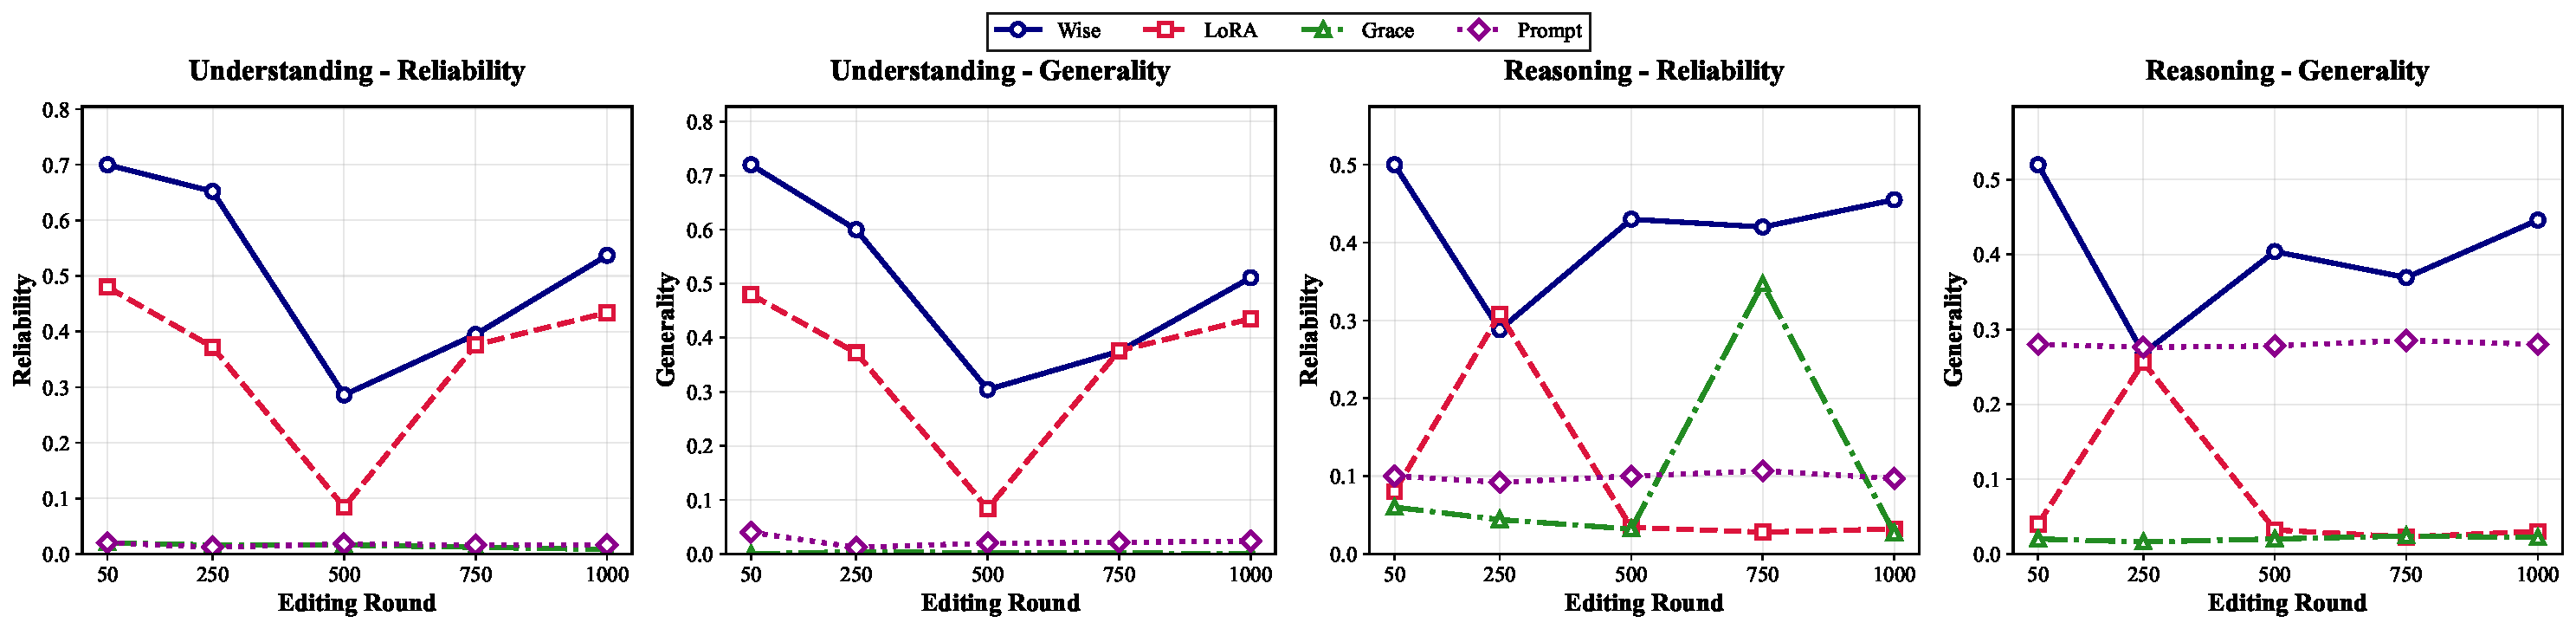
\includegraphics[width=\linewidth]{Figures/LifeLong_Huatuo.pdf}
   \caption{Lifelong editing performance of HuatuoGPT-7B using different editing approaches (Wise, LoRA, Grace, Prompt). The figure reports Reliability and Generality scores on both \textit{understanding} and \textit{reasoning} tasks under varying numbers of edits.}

    \label{fig:LifeLong}
\end{figure*}

\section{Appendix C: Lifelong Edit on HuatuoGPT-7B}
The Lifelong Edit Result on HuatuoGPT-7B is shown in Figure~\ref{fig:LifeLong}. For all methods across both understanding and reasoning tasks, T-Locality and M-Locality remain consistently high (mostly above 0.8 or even 1.0), indicating that the edits are well-localized both in terms of task and memory, with minimal unintended interference.






\section{Appendix D: Benchmark Construction Details}
The prompt templates are as shown in Figure \ref{fig:PromptRephrase}.


\section{Appendix E: Samples from MultiMedBench}
Representative cases from MultiMedBench are illustrated in Figure~\ref{fig:CaseDataUnderstanding} and Figure~\ref{fig:CaseDataReasoning}, covering both understanding and reasoning tasks. We have selected 50 examples for each category, which are included in the accompanying ZIP file.





\begin{figure*}[htp]
    \centering
   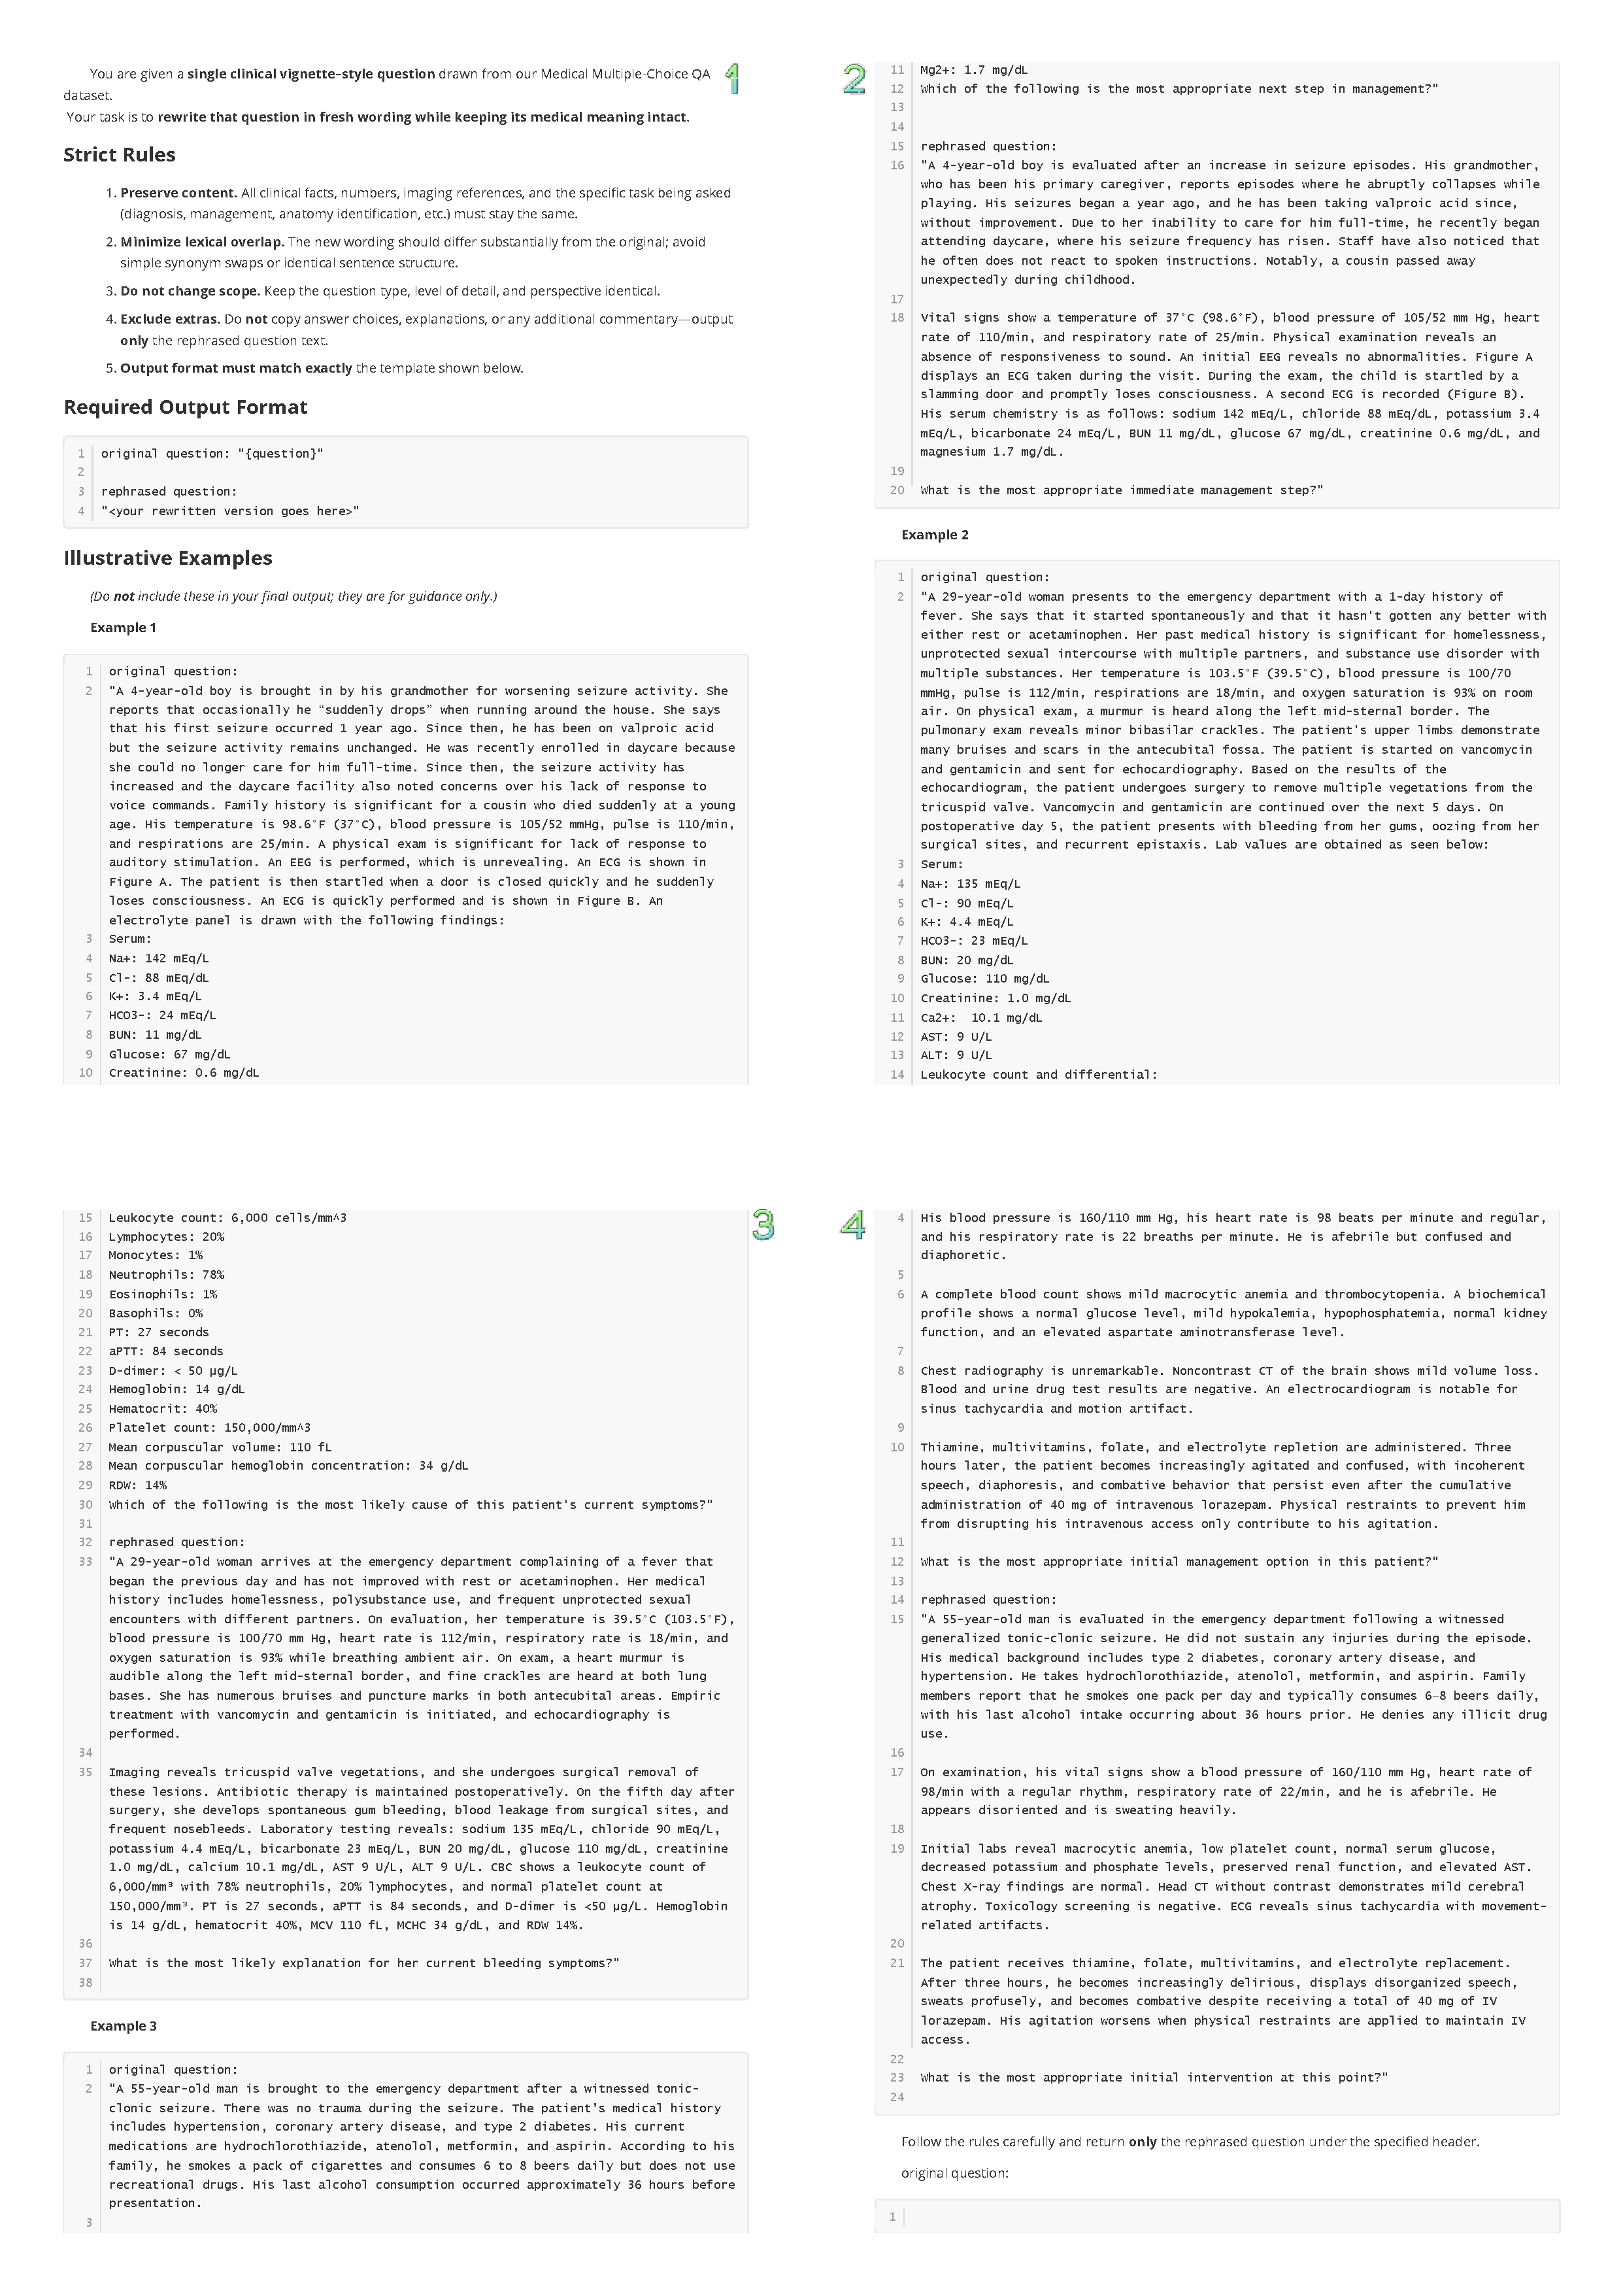
\includegraphics[scale=0.38]{Figures/PromptRephrase.pdf}
    \caption{Prompt template of question rephrase.}
    \label{fig:PromptRephrase}
\end{figure*}


\begin{figure*}[htp]
    \centering
   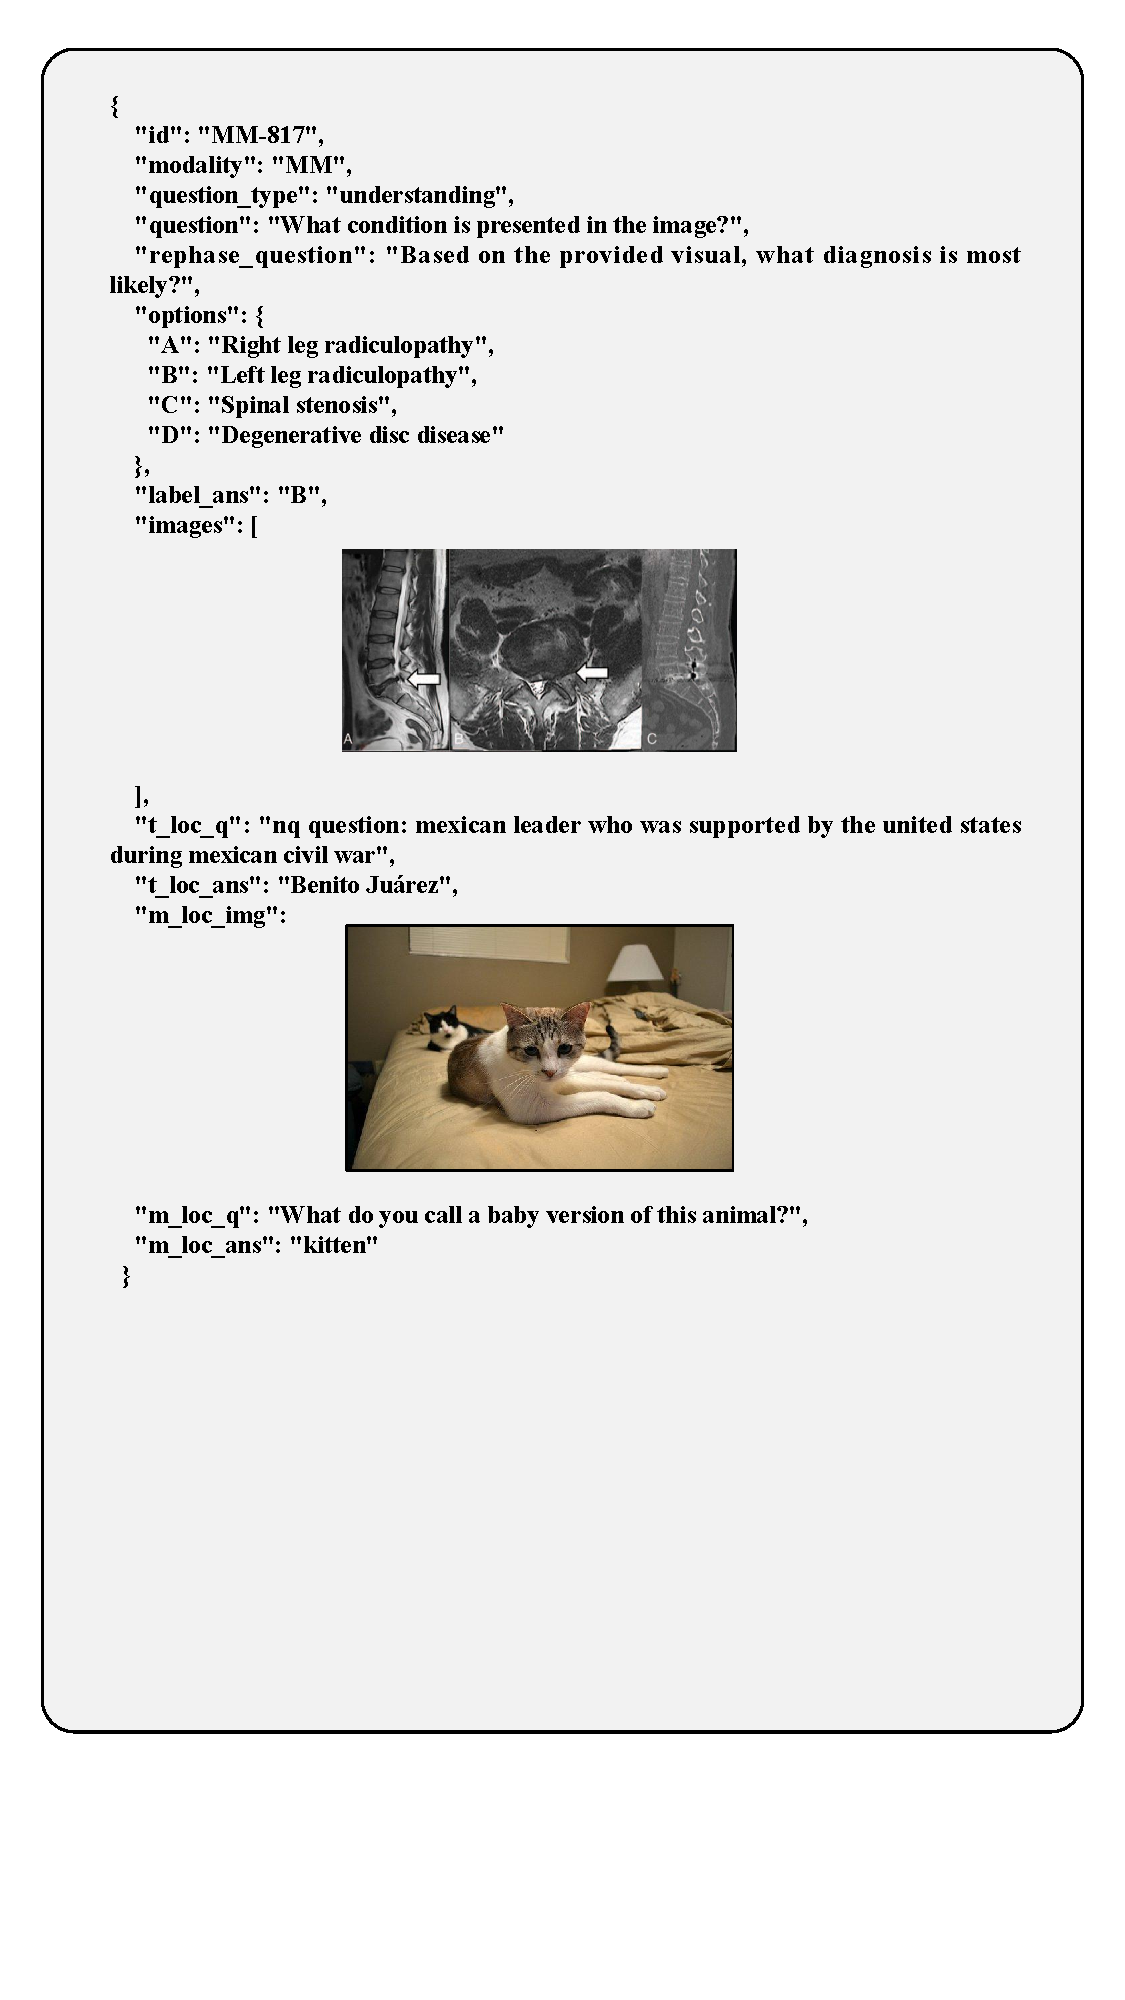
\includegraphics[scale=0.7]{Figures/CaseData-Understanding.pdf}
    \caption{Prompt template of question rephrase.}
    \label{fig:CaseDataUnderstanding}
\end{figure*}



\begin{figure*}[htp]
    \centering
   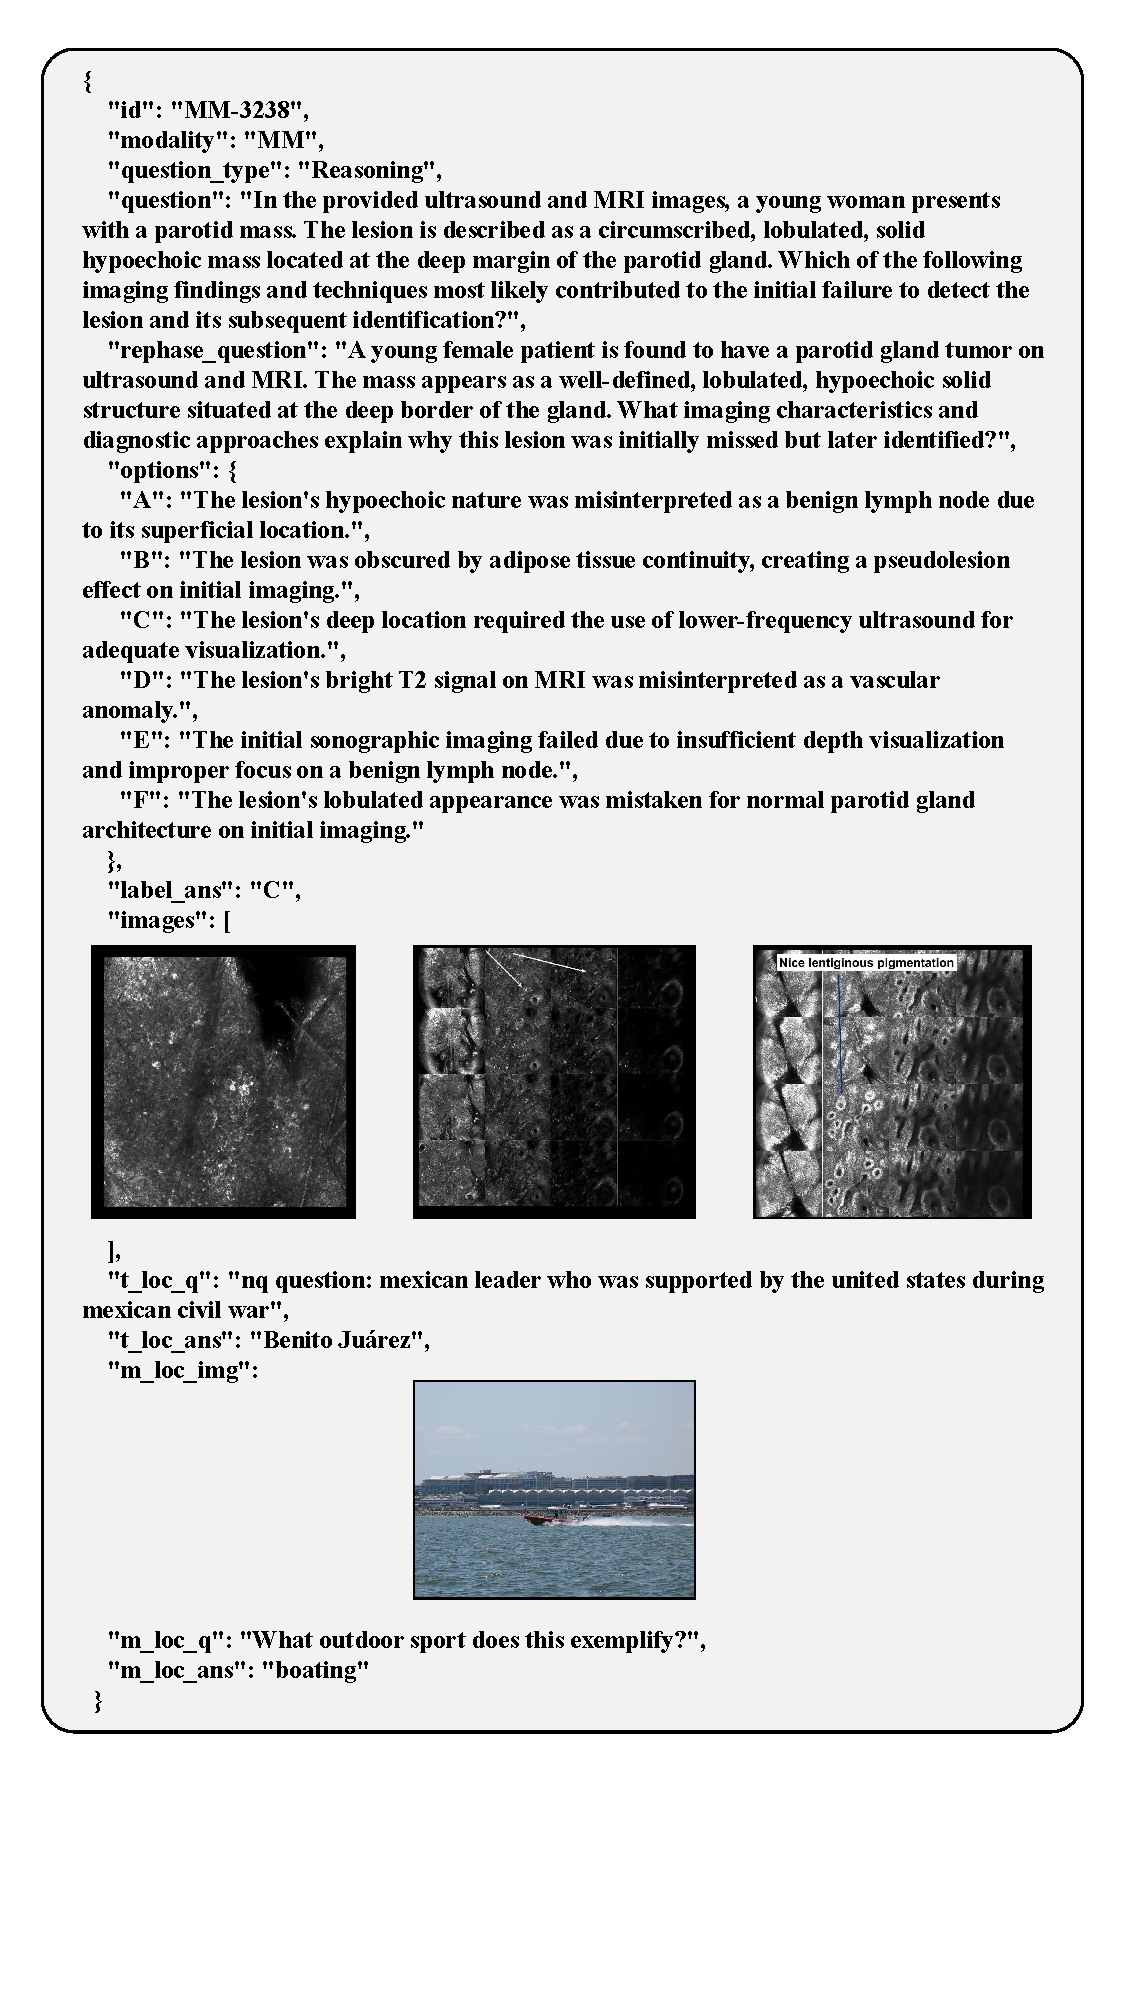
\includegraphics[scale=0.7]{Figures/CaseData-Reasoning.pdf}
    \caption{Prompt template of question rephrase.}
    \label{fig:CaseDataReasoning}
\end{figure*}









% \bibliography{aaai2026}
\end{document}
